\documentclass{standalone}
\usepackage{tikz}
\usetikzlibrary{patterns, positioning}


\begin{document}
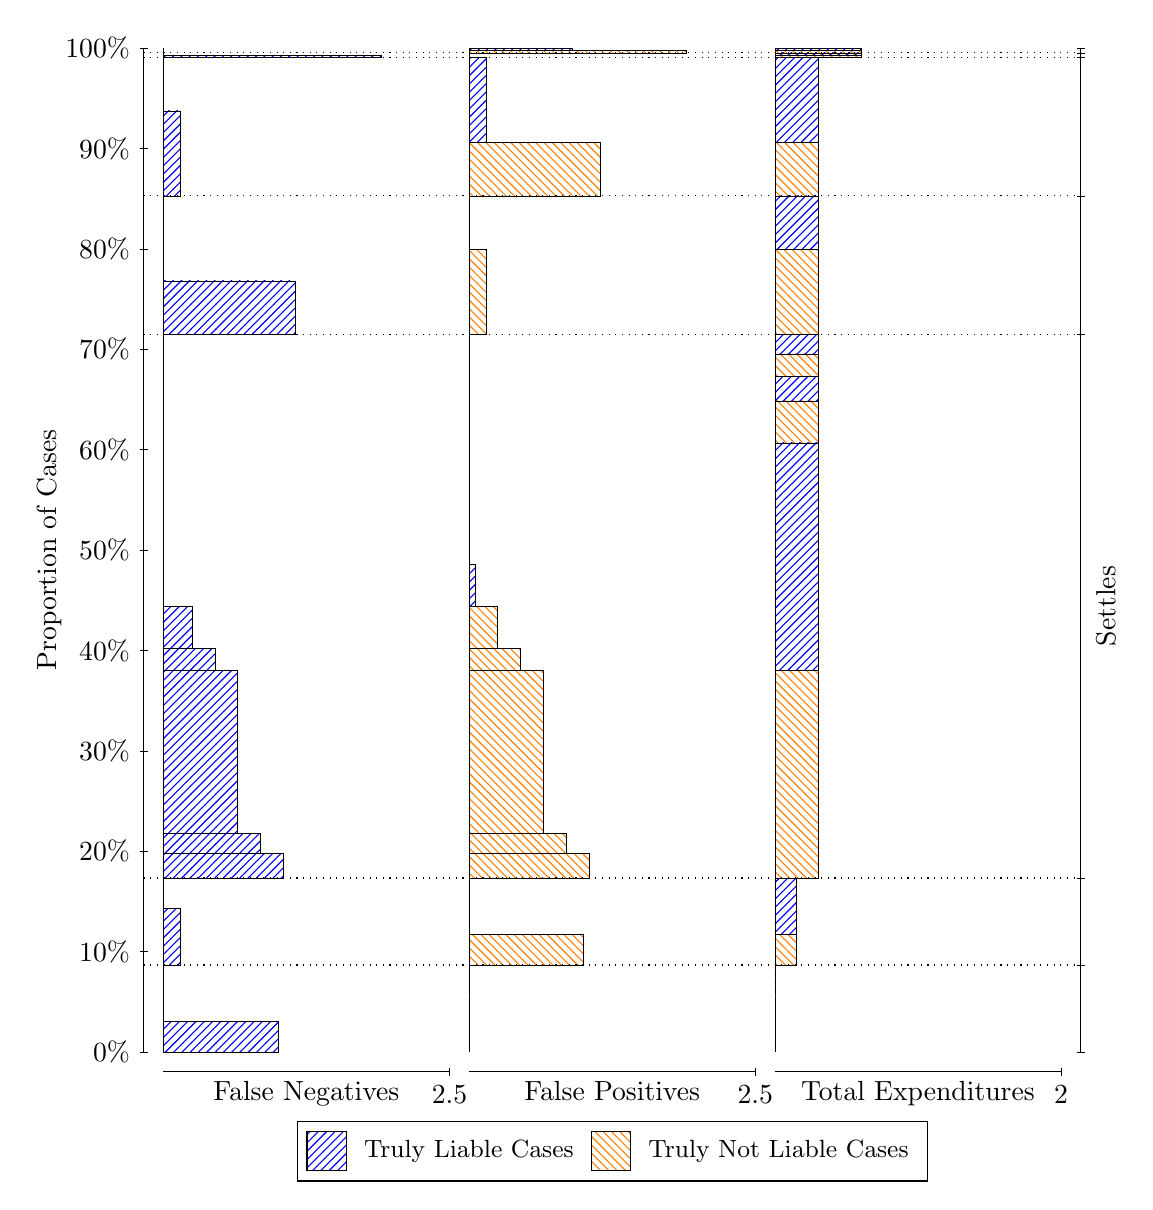
\begin{tikzpicture}
\draw[black, very thin] (1.5,1.75) -- (1.5,14.5);
\node[rotate=90, text=black, anchor=center] at (0.3, 8.125) {Proportion of Cases};
\draw[black, very thin] (1.45,1.75) -- (1.55,1.75);
\node[text=black, anchor=east] at (1.45, 1.75) {0\%};
\draw[black, very thin] (1.45,3.025) -- (1.55,3.025);
\node[text=black, anchor=east] at (1.45, 3.025) {10\%};
\draw[black, very thin] (1.45,4.3) -- (1.55,4.3);
\node[text=black, anchor=east] at (1.45, 4.3) {20\%};
\draw[black, very thin] (1.45,5.575) -- (1.55,5.575);
\node[text=black, anchor=east] at (1.45, 5.575) {30\%};
\draw[black, very thin] (1.45,6.85) -- (1.55,6.85);
\node[text=black, anchor=east] at (1.45, 6.85) {40\%};
\draw[black, very thin] (1.45,8.125) -- (1.55,8.125);
\node[text=black, anchor=east] at (1.45, 8.125) {50\%};
\draw[black, very thin] (1.45,9.4) -- (1.55,9.4);
\node[text=black, anchor=east] at (1.45, 9.4) {60\%};
\draw[black, very thin] (1.45,10.675) -- (1.55,10.675);
\node[text=black, anchor=east] at (1.45, 10.675) {70\%};
\draw[black, very thin] (1.45,11.95) -- (1.55,11.95);
\node[text=black, anchor=east] at (1.45, 11.95) {80\%};
\draw[black, very thin] (1.45,13.225) -- (1.55,13.225);
\node[text=black, anchor=east] at (1.45, 13.225) {90\%};
\draw[black, very thin] (1.45,14.5) -- (1.55,14.5);
\node[text=black, anchor=east] at (1.45, 14.5) {100\%};

\draw[black, very thin] (13.4,1.75) -- (13.4,14.5);
\draw[black, very thin] (13.35,1.75) -- (13.45,1.75);
\node[anchor=west] at (13.35, 1.75) {};
\draw[black, very thin] (13.35,2.8545) -- (13.45,2.8545);
\node[anchor=west] at (13.35, 2.8545) {};
\draw[black, very thin] (13.35,3.9589) -- (13.45,3.9589);
\node[anchor=west] at (13.35, 3.9589) {};
\draw[black, very thin] (13.35,10.866) -- (13.45,10.866);
\node[anchor=west] at (13.35, 10.866) {};
\draw[black, very thin] (13.35,12.622) -- (13.45,12.622);
\node[anchor=west] at (13.35, 12.622) {};
\draw[black, very thin] (13.35,14.378) -- (13.45,14.378);
\node[anchor=west] at (13.35, 14.378) {};
\draw[black, very thin] (13.35,14.439) -- (13.45,14.439);
\node[anchor=west] at (13.35, 14.439) {};
\draw[black, very thin] (13.35,14.5) -- (13.45,14.5);
\node[anchor=west] at (13.35, 14.5) {};

\draw[black, very thin, pattern color=blue, pattern=north east lines] (1.75,1.75) rectangle (3.2033,2.1392);
\draw[black, very thin, pattern color=orange, pattern=north west lines] (1.75,2.1392) rectangle (1.75,2.8545);
\draw[black, very thin, pattern color=blue, pattern=north east lines] (1.75,2.8545) rectangle (1.968,3.5697);
\draw[black, very thin, pattern color=orange, pattern=north west lines] (1.75,3.5697) rectangle (1.75,3.9589);
\draw[black, very thin, pattern color=blue, pattern=north east lines] (1.75,3.9589) rectangle (3.276,4.2742);
\draw[black, very thin, pattern color=blue, pattern=north east lines] (1.75,4.2742) rectangle (2.9853,4.5245);
\draw[black, very thin, pattern color=blue, pattern=north east lines] (1.75,4.5245) rectangle (2.6947,6.5966);
\draw[black, very thin, pattern color=blue, pattern=north east lines] (1.75,6.5966) rectangle (2.404,6.8784);
\draw[black, very thin, pattern color=blue, pattern=north east lines] (1.75,6.8784) rectangle (2.1133,7.4124);
\draw[black, very thin, pattern color=orange, pattern=north west lines] (1.75,7.4124) rectangle (1.75,10.866);
\draw[black, very thin, pattern color=blue, pattern=north east lines] (1.75,10.866) rectangle (3.4213,11.542);
\draw[black, very thin, pattern color=orange, pattern=north west lines] (1.75,11.542) rectangle (1.75,12.622);
\draw[black, very thin, pattern color=blue, pattern=north east lines] (1.75,12.622) rectangle (1.968,13.702);
\draw[black, very thin, pattern color=orange, pattern=north west lines] (1.75,13.702) rectangle (1.75,14.378);
\draw[black, very thin, pattern color=blue, pattern=north east lines] (1.75,14.378) rectangle (4.5113,14.405);
\draw[black, very thin, pattern color=orange, pattern=north west lines] (1.75,14.405) rectangle (1.75,14.439);
\draw[black, very thin, pattern color=orange, pattern=north west lines] (1.75,14.439) rectangle (1.75,14.466);
\draw[black, very thin, pattern color=blue, pattern=north east lines] (1.75,14.466) rectangle (1.75,14.5);
\draw[black, very thin, pattern color=orange, pattern=north west lines] (5.6333,1.75) rectangle (5.6333,2.4652);
\draw[black, very thin, pattern color=blue, pattern=north east lines] (5.6333,2.4652) rectangle (5.6333,2.8545);
\draw[black, very thin, pattern color=orange, pattern=north west lines] (5.6333,2.8545) rectangle (7.0867,3.2437);
\draw[black, very thin, pattern color=blue, pattern=north east lines] (5.6333,3.2437) rectangle (5.6333,3.9589);
\draw[black, very thin, pattern color=orange, pattern=north west lines] (5.6333,3.9589) rectangle (7.1593,4.2742);
\draw[black, very thin, pattern color=orange, pattern=north west lines] (5.6333,4.2742) rectangle (6.8687,4.5245);
\draw[black, very thin, pattern color=orange, pattern=north west lines] (5.6333,4.5245) rectangle (6.578,6.5966);
\draw[black, very thin, pattern color=orange, pattern=north west lines] (5.6333,6.5966) rectangle (6.2873,6.8784);
\draw[black, very thin, pattern color=orange, pattern=north west lines] (5.6333,6.8784) rectangle (5.9967,7.4124);
\draw[black, very thin, pattern color=blue, pattern=north east lines] (5.6333,7.4124) rectangle (5.706,7.9464);
\draw[black, very thin, pattern color=blue, pattern=north east lines] (5.6333,7.9464) rectangle (5.6333,10.866);
\draw[black, very thin, pattern color=orange, pattern=north west lines] (5.6333,10.866) rectangle (5.8513,11.946);
\draw[black, very thin, pattern color=blue, pattern=north east lines] (5.6333,11.946) rectangle (5.6333,12.622);
\draw[black, very thin, pattern color=orange, pattern=north west lines] (5.6333,12.622) rectangle (7.3047,13.298);
\draw[black, very thin, pattern color=blue, pattern=north east lines] (5.6333,13.298) rectangle (5.8513,14.378);
\draw[black, very thin, pattern color=orange, pattern=north west lines] (5.6333,14.378) rectangle (5.6333,14.412);
\draw[black, very thin, pattern color=blue, pattern=north east lines] (5.6333,14.412) rectangle (5.6333,14.439);
\draw[black, very thin, pattern color=orange, pattern=north west lines] (5.6333,14.439) rectangle (8.3947,14.466);
\draw[black, very thin, pattern color=blue, pattern=north east lines] (5.6333,14.466) rectangle (6.9413,14.5);
\draw[black, very thin, pattern color=orange, pattern=north west lines] (9.5167,1.75) rectangle (9.5167,2.4652);
\draw[black, very thin, pattern color=blue, pattern=north east lines] (9.5167,2.4652) rectangle (9.5167,2.8545);
\draw[black, very thin, pattern color=orange, pattern=north west lines] (9.5167,2.8545) rectangle (9.7892,3.2437);
\draw[black, very thin, pattern color=blue, pattern=north east lines] (9.5167,3.2437) rectangle (9.7892,3.9589);
\draw[black, very thin, pattern color=orange, pattern=north west lines] (9.5167,3.9589) rectangle (10.062,6.5966);
\draw[black, very thin, pattern color=blue, pattern=north east lines] (9.5167,6.5966) rectangle (10.062,9.4844);
\draw[black, very thin, pattern color=orange, pattern=north west lines] (9.5167,9.4844) rectangle (10.062,10.018);
\draw[black, very thin, pattern color=blue, pattern=north east lines] (9.5167,10.018) rectangle (10.062,10.334);
\draw[black, very thin, pattern color=orange, pattern=north west lines] (9.5167,10.334) rectangle (10.062,10.616);
\draw[black, very thin, pattern color=blue, pattern=north east lines] (9.5167,10.616) rectangle (10.062,10.866);
\draw[black, very thin, pattern color=orange, pattern=north west lines] (9.5167,10.866) rectangle (10.062,11.946);
\draw[black, very thin, pattern color=blue, pattern=north east lines] (9.5167,11.946) rectangle (10.062,12.622);
\draw[black, very thin, pattern color=orange, pattern=north west lines] (9.5167,12.622) rectangle (10.062,13.298);
\draw[black, very thin, pattern color=blue, pattern=north east lines] (9.5167,13.298) rectangle (10.062,14.378);
\draw[black, very thin, pattern color=orange, pattern=north west lines] (9.5167,14.378) rectangle (10.607,14.412);
\draw[black, very thin, pattern color=blue, pattern=north east lines] (9.5167,14.412) rectangle (10.607,14.439);
\draw[black, very thin, pattern color=orange, pattern=north west lines] (9.5167,14.439) rectangle (10.607,14.466);
\draw[black, very thin, pattern color=blue, pattern=north east lines] (9.5167,14.466) rectangle (10.607,14.5);
\draw[black, dotted] (1.5,2.8545) -- (13.4,2.8545);
\draw[black, dotted] (1.5,3.9589) -- (13.4,3.9589);
\draw[black, dotted] (1.5,10.866) -- (13.4,10.866);
\draw[black, dotted] (1.5,12.622) -- (13.4,12.622);
\draw[black, dotted] (1.5,14.378) -- (13.4,14.378);
\draw[black, dotted] (1.5,14.439) -- (13.4,14.439);
\draw[black, very thin] (1.75,1.5) -- (5.3833,1.5);
\node[text=black, anchor=north] at (3.5667, 1.5) {False Negatives};
\draw[black, very thin] (5.3833,1.45) -- (5.3833,1.55);
\node[text=black, anchor=north] at (5.3833, 1.45) {2.5};

\draw[black, very thin] (5.6333,1.5) -- (9.2667,1.5);
\node[text=black, anchor=north] at (7.45, 1.5) {False Positives};
\draw[black, very thin] (9.2667,1.45) -- (9.2667,1.55);
\node[text=black, anchor=north] at (9.2667, 1.45) {2.5};

\draw[black, very thin] (9.5167,1.5) -- (13.15,1.5);
\node[text=black, anchor=north] at (11.333, 1.5) {Total Expenditures};
\draw[black, very thin] (13.15,1.45) -- (13.15,1.55);
\node[text=black, anchor=north] at (13.15, 1.45) {2};



\node[text=black, centered, rotate=90] at (13.72, 7.4124) {Settles};





\draw (7.449999999999999,1.5) node[draw=none] (baseCoordinate) {};
\begin{scope}[align=center]
        \matrix[scale=0.5, draw=black, below=0.5cm of baseCoordinate, nodes={draw}, column sep=0.1cm]{
            \node[rectangle, draw, minimum width=0.5cm, minimum height=0.5cm, pattern color=blue, pattern=north east lines] {}; &
            \node[draw=none, font=\small, text=black] (B) {Truly Liable Cases}; &
            \node[rectangle, draw, minimum width=0.5cm, minimum height=0.5cm, pattern color=orange, pattern=north west lines] {}; &
            \node[draw=none, font=\small, text=black] (B) {Truly Not Liable Cases}; \\
            };
\end{scope}

\end{tikzpicture}
\end{document}